% Chapter 12: Applications

\chapter{Applications}
\label{chap:applications}

This chapter showcases deep learning applications across various domains, demonstrating the breadth and impact of the field.


\section*{Learning Objectives}
\addcontentsline{toc}{section}{Learning Objectives}

After studying this chapter, you will be able to:

\begin{enumerate}
    \item Identify opportunities where deep learning provides value in vision, language, speech, and tabular domains.
    \item Select appropriate model families and data representations for each application area.
    \item Design evaluation protocols and metrics suited to each task type.
    \item Recognize common failure modes and deployment considerations across applications.
\end{enumerate}



\section*{Intuition}
\addcontentsline{toc}{section}{Intuition}

Applications differ not only in architectures but in \emph{data assumptions and metrics}. A robust recipe is: clarify the task and loss, understand the data distribution and constraints, then choose the simplest model that can plausibly meet the requirements before scaling up.


% Chapter 12, Section 1

\section{Computer Vision Applications \difficultyInline{beginner}}
\label{sec:cv-applications}

\subsection{Image Classification}

Assign labels to images; modern benchmarks like ImageNet catalyzed deep CNN adoption \index{ImageNet} \textcite{Krizhevsky2012,He2016,GoodfellowEtAl2016,Prince2023}.
\begin{itemize}
    \item \textbf{ImageNet:} 1000-class object recognition
    \item \textbf{Fine-grained classification:} Bird species, car models
    \item \textbf{Medical imaging:} Disease classification from X-rays, CT scans
\end{itemize}

\textbf{Architecture:} CNN backbone (e.g., ResNet) + classification head; transfer learning from pretrained weights is standard practice.

\begin{figure}[h]
  \centering
  \begin{tikzpicture}[>=stealth]
    \tikzstyle{block}=[draw,rounded corners,align=center,minimum width=2.2cm,minimum height=0.9cm]
    \node[block,fill=bookpurple!10] at (0,0) (img) {Input Image};
    \node[block,fill=bookpurple!15] at (3.2,0) (conv) {Conv\,/\,BN\,/\,ReLU $\times N$};
    \node[block,fill=bookpurple!20] at (6.4,0) (pool) {Global Avg Pool};
    \node[block,fill=bookpurple!25] at (9.6,0) (fc) {Fully Connected};
    \node[block,fill=bookpurple!30] at (12.8,0) (softmax) {Softmax};
    \draw[->] (img) -- (conv);
    \draw[->] (conv) -- (pool);
    \draw[->] (pool) -- (fc);
    \draw[->] (fc) -- (softmax);
  \end{tikzpicture}
  \caption{Typical CNN classification pipeline.}
  \label{fig:cnn-pipeline}
\end{figure}

\subsection{Object Detection}

Locate and classify objects in images; real-time variants (YOLO) emphasize speed, while two-stage models (Faster R-CNN) emphasize accuracy.
\begin{itemize}
    \item \textbf{Autonomous driving:} Pedestrians, vehicles, traffic signs
    \item \textbf{Surveillance:} Person detection and tracking
    \item \textbf{Retail:} Product recognition
\end{itemize}

\textbf{Methods:} YOLO, Faster R-CNN, RetinaNet; focal loss handles class imbalance in dense detectors.

\begin{figure}[h]
  \centering
  \begin{tikzpicture}
    \begin{axis}[
      width=0.48\textwidth,height=0.36\textwidth,
      xlabel={IoU threshold}, ylabel={mAP}, grid=both]
      \addplot[bookpurple,very thick] coordinates{(0.5,0.60) (0.55,0.58) (0.6,0.55) (0.65,0.52) (0.7,0.48) (0.75,0.43)};
    \end{axis}
  \end{tikzpicture}
  \caption{Detector performance (mAP) vs. IoU threshold schematic.}
  \label{fig:map-iou}
\end{figure}

\subsection{Semantic Segmentation}

Classify every pixel:
\begin{itemize}
    \item \textbf{Autonomous driving:} Road, sidewalk, vehicle segmentation
    \item \textbf{Medical imaging:} Tumor segmentation, organ delineation
    \item \textbf{Satellite imagery:} Land use classification
\end{itemize}

\textbf{Architectures:} U-Net, DeepLab, Mask R-CNN

\begin{figure}[h]
  \centering
  \begin{tikzpicture}
    \tikzstyle{enc}=[draw,rounded corners,fill=bookpurple!10,minimum width=1.2cm,minimum height=0.7cm]
    \tikzstyle{dec}=[draw,rounded corners,fill=bookred!10,minimum width=1.2cm,minimum height=0.7cm]
    % Encoder blocks
    \node[enc] at (0,0) (e1) {E1};
    \node[enc] at (2.0,0) (e2) {E2};
    \node[enc] at (4.0,0) (e3) {E3};
    % Decoder blocks
    \node[dec] at (3.0,1.4) (d2) {D2};
    \node[dec] at (1.0,2.6) (d1) {D1};
    % Connections
    \draw[->] (e1) -- (e2);
    \draw[->] (e2) -- (e3);
    \draw[->] (e3) |- (d2);
    \draw[->] (d2) |- (d1);
    % Skip connections
    \draw (e2.north) -- (d2.south);
    \draw (e1.north) -- (d1.south);
  \end{tikzpicture}
  \caption{U-Net style encoder-decoder with skip connections.}
  \label{fig:unet-schematic}
\end{figure}

\subsection{Face Recognition}

Identify or verify individuals:
\begin{itemize}
    \item Security and access control
    \item Photo organization
    \item Payment authentication
\end{itemize}

\textbf{Approach:} Face detection + embedding (FaceNet, ArcFace) + similarity matching; report ROC/PR, false accept/reject at target FAR/FRR.

\subsection{Image Generation and Manipulation}

\begin{itemize}
    \item \textbf{Style transfer:} Apply artistic styles
    \item \textbf{Super-resolution:} Enhance image quality
    \item \textbf{Inpainting:} Fill missing regions
    \item \textbf{Deepfakes:} Face swapping (ethical concerns)
\end{itemize}

\subsection{Historical context and references}

Modern CV breakthroughs stem from CNNs popularized by ImageNet-scale training \textcite{Krizhevsky2012}, deeper residual networks \textcite{He2016}, and specialized architectures for segmentation \textcite{Ronneberger2015}. See \textcite{GoodfellowEtAl2016,Prince2023} for broader context.

% Chapter 12, Section 2

\section{Natural Language Processing \difficultyInline{beginner}}
\label{sec:nlp-applications}

Natural Language Processing represents one of the most widely adopted applications of deep learning, transforming how humans interact with computers through text and speech. From search engines that understand natural language queries to virtual assistants that can engage in meaningful conversations, NLP has become an integral part of modern digital experiences. The field has experienced revolutionary advances with the introduction of transformer architectures and large language models, enabling applications that were previously impossible, such as real-time translation between hundreds of languages and AI systems that can generate human-like text. These technologies power everything from customer service chatbots and content recommendation systems to advanced research tools and educational platforms, making NLP one of the most impactful areas of artificial intelligence in terms of daily user interaction and business value.

\subsection{Text Classification}

Text classification serves as the foundation for many NLP applications, automatically categorizing documents and messages to enable intelligent routing, filtering, and analysis. This technology has become essential for managing the vast amounts of textual data generated daily across digital platforms, from social media posts and customer feedback to legal documents and scientific papers.

Sentiment analysis applications analyze the emotional tone and opinion expressed in text, enabling businesses to monitor customer satisfaction, track brand perception, and respond to public sentiment in real-time. Social media platforms use this technology to detect hate speech and harmful content, while e-commerce sites analyze product reviews to provide sentiment-based recommendations and identify trending items. Financial institutions employ sentiment analysis to gauge market sentiment from news articles and social media, helping traders make informed investment decisions. The technology is also used in political campaigns to understand public opinion and in healthcare to monitor patient satisfaction and mental health indicators from text communications.

Spam detection systems protect users from unwanted and potentially harmful messages by automatically identifying and filtering spam emails, phishing attempts, and malicious content. Email providers use sophisticated NLP models to achieve near-perfect spam detection rates while minimizing false positives that might block legitimate messages. Social media platforms employ similar technology to detect and remove spam accounts, fake reviews, and malicious content that could harm users or manipulate public opinion. The technology has evolved to handle increasingly sophisticated spam techniques, including AI-generated content and context-aware attacks that traditional rule-based systems cannot detect.

Topic classification systems automatically organize large collections of documents by subject matter, enabling efficient information retrieval and content management. News organizations use this technology to automatically categorize articles by topic, making it easier for readers to find relevant content and for editors to manage their content libraries. Academic institutions employ topic classification to organize research papers and help researchers discover relevant studies in their fields. Legal firms use the technology to categorize case documents and contracts, while government agencies apply it to process and organize public records and regulatory documents.

Modern text classification systems typically use pretrained transformer models like BERT, RoBERTa, and DistilBERT, which can be fine-tuned for specific tasks with relatively small amounts of domain-specific data. These models achieve state-of-the-art performance across diverse classification tasks while being computationally efficient enough for real-time applications. Evaluation metrics include accuracy and F1 scores for general applications, while risk-sensitive domains like healthcare and finance require additional attention to model calibration to ensure that confidence scores accurately reflect prediction reliability. The success of these models has made advanced text classification capabilities accessible to organizations of all sizes, democratizing access to sophisticated NLP technology.

\begin{figure}[h]
  \centering
  \begin{tikzpicture}
    \tikzstyle{b}=[draw,rounded corners,align=center,minimum width=2.3cm,minimum height=0.9cm]
    \node[b,fill=bookpurple!10] at (0,0) (tok) {Tokenize +\newline Embed};
    \node[b,fill=bookpurple!15] at (3.0,0) (enc) {Transformer\newline Encoder ($L$ layers)};
    \node[b,fill=bookpurple!20] at (6.0,0) (cls) {[CLS] pooled};
    \node[b,fill=bookpurple!30] at (9.0,0) (head) {Softmax head};
    \draw[->] (tok) -- (enc);
    \draw[->] (enc) -- (cls);
    \draw[->] (cls) -- (head);
  \end{tikzpicture}
  \caption{Transformer fine-tuning for text classification.}
  \label{fig:nlp-class}
\end{figure}

\subsection{Machine Translation}

Machine translation represents one of the most transformative applications of NLP, breaking down language barriers and enabling global communication on an unprecedented scale. The technology has evolved from rule-based systems to statistical methods and finally to neural approaches that can translate between hundreds of language pairs with remarkable accuracy. Modern translation systems can handle complex linguistic phenomena, cultural nuances, and domain-specific terminology, making them essential tools for international business, education, and diplomacy. The introduction of attention mechanisms and transformer architectures revolutionized the field, enabling translations that often rival human quality while being fast enough for real-time applications.

Google Translate and DeepL represent the most widely used commercial translation services, processing billions of translation requests daily across diverse applications. Google Translate supports over 100 languages and is integrated into search results, email, and mobile apps, enabling users to understand content in foreign languages instantly. DeepL has gained recognition for its high-quality translations, particularly for European languages, and is widely used by professionals who require accurate translations for business documents and academic papers. These services power everything from tourist apps that translate signs and menus to e-commerce platforms that automatically translate product descriptions for international markets.

Sequence-to-sequence models with attention mechanisms revolutionized machine translation by enabling the model to focus on relevant parts of the source sentence when generating each word of the translation. This approach solved the bottleneck problem of earlier encoder-decoder architectures, allowing the model to handle long sentences and complex linguistic structures effectively. The attention mechanism enables the model to learn alignment between source and target languages, making translations more accurate and contextually appropriate. These models are particularly effective for languages with different word orders and grammatical structures, enabling high-quality translation between linguistically distant language pairs.

Transformer models have become the standard architecture for machine translation, offering superior performance and efficiency compared to earlier recurrent neural network approaches. These models can be trained on massive parallel corpora, learning to translate between multiple language pairs simultaneously while sharing knowledge across languages. The self-attention mechanism allows the model to capture long-range dependencies and complex linguistic patterns that are essential for accurate translation. Modern transformer-based translation systems can handle specialized domains like legal, medical, and technical texts, making them valuable tools for professional translators and international organizations.

Modern machine translation architectures use encoder-decoder transformers with subword tokenization to handle the vocabulary size and morphological complexity of different languages. The encoder processes the source language text to create contextual representations, while the decoder generates the target language text using cross-attention to focus on relevant source information. Subword tokenization enables the model to handle rare words and morphological variations effectively, improving translation quality for languages with rich morphology. Evaluation uses metrics like BLEU and chrF for automated assessment, combined with human evaluation to measure translation quality, fluency, and cultural appropriateness. These systems have achieved near-human performance on many language pairs, making real-time translation practical for applications like video conferencing, live streaming, and international communication.

\begin{figure}[h]
  \centering
  \begin{tikzpicture}
    \tikzstyle{e}=[draw,rounded corners,fill=bookpurple!10,minimum width=1.8cm,minimum height=0.7cm]
    \tikzstyle{d}=[draw,rounded corners,fill=bookred!10,minimum width=1.8cm,minimum height=0.7cm]
    \node[e] at (0,0) (e1) {Enc 1};
    \node[e] at (2.1,0) (e2) {Enc 2};
    \node[e] at (4.2,0) (e3) {Enc 3};
    \node[d] at (2.1,1.6) (d1) {Dec 1};
    \node[d] at (4.2,1.6) (d2) {Dec 2};
    \draw[->] (e1) -- (e2);
    \draw[->] (e2) -- (e3);
    \draw[->] (e3) -- (d2);
    \draw[->] (d1) -- (d2);
    \draw (e2.north) -- (d1.south);
  \end{tikzpicture}
  \caption{Encoder–decoder Transformer schematic with cross-attention.}
  \label{fig:mt-transformer}
\end{figure}

\subsection{Question Answering}

Question answering systems represent one of the most challenging and valuable applications of NLP, enabling users to obtain specific information by asking natural language questions. These systems must understand the semantic meaning of questions, locate relevant information from vast knowledge sources, and generate accurate, coherent answers that directly address the user's query. The technology has evolved from simple keyword matching to sophisticated neural models that can reason about complex relationships and provide nuanced answers to diverse question types. Modern QA systems are essential components of search engines, virtual assistants, and educational platforms, transforming how people access and interact with information.

Extractive question answering systems find the answer span within a given text passage, making them particularly effective for applications where the answer exists verbatim in the source material. The SQuAD dataset has become the standard benchmark for this task, enabling systems to answer questions like "What is the capital of France?" by locating the relevant text span. These systems are widely used in customer service applications where agents need to quickly find answers from knowledge bases, in legal research where lawyers search through case documents, and in educational platforms where students can ask questions about course materials. The technology is also valuable for fact-checking applications that need to verify claims against reliable sources and for research tools that help scientists find relevant information in academic papers.

Open-domain question answering systems can answer questions by searching through large corpora of text, including the entire internet, making them incredibly powerful tools for information retrieval. These systems combine information retrieval techniques with reading comprehension models to first find relevant documents and then extract or generate answers from them. They power modern search engines that can provide direct answers to questions rather than just returning lists of relevant web pages. The technology is used in virtual assistants like Siri and Alexa to answer general knowledge questions, in educational platforms to help students with homework and research, and in professional tools that help researchers and analysts find information quickly. These systems are particularly valuable for applications that require up-to-date information, as they can access the latest content from the web.

Visual question answering systems combine computer vision and natural language processing to answer questions about images, enabling applications that can understand and describe visual content. These systems can answer questions like "What color is the car?" or "How many people are in the image?" by analyzing both the visual content and the linguistic structure of the question. The technology is used in accessibility applications that help visually impaired users understand images, in educational tools that can answer questions about diagrams and illustrations, and in content moderation systems that can understand the context of images to detect inappropriate content. These systems are also valuable for medical imaging applications where doctors can ask questions about X-rays or scans to get AI-assisted diagnostic insights.

\subsection{Language Models and Text Generation}

Large language models represent the most transformative development in NLP, enabling AI systems to generate human-like text across diverse applications and domains. These models have revolutionized how we interact with computers, enabling natural language interfaces that can understand context, maintain conversation flow, and provide helpful responses to complex queries. The technology has achieved remarkable capabilities in text generation, from creative writing and technical documentation to code generation and educational content creation. However, the power of these models also raises important considerations about safety, accuracy, and responsible deployment, requiring careful evaluation and human oversight to ensure they provide reliable and beneficial assistance.

GPT models have become the most widely used large language models for general text generation, with ChatGPT/OpenAI holding approximately 80% market share as of October 2025. These models power everything from creative writing assistants that help authors develop story ideas and dialogue to educational tools that can explain complex concepts in simple terms. The technology is used in content marketing to generate blog posts and social media content, in customer service to provide automated responses that feel natural and helpful, and in research applications to summarize papers and generate hypotheses. The models' ability to understand context and maintain coherence across long passages makes them valuable for applications that require sustained, meaningful interaction with users.

Code generation applications like GitHub Copilot, Gemini, Revo, and Codex have transformed software development by providing AI-powered coding assistance that can understand natural language descriptions and generate corresponding code. These tools can suggest function implementations, debug code, write tests, and even generate entire applications from high-level specifications. Developers use these systems to accelerate their workflow, learn new programming languages, and explore different approaches to solving problems. The technology is particularly valuable for educational applications where students can learn programming concepts through interactive AI assistance, and for professional development where engineers can quickly prototype ideas and explore new technologies. These systems have become essential tools for modern software development, enabling faster iteration and more creative problem-solving.

Chatbots and conversational AI systems have become ubiquitous in customer service, education, and entertainment applications, providing 24/7 assistance that can handle a wide range of user queries. These systems power virtual assistants that can help with scheduling, information retrieval, and task automation, making them valuable tools for personal productivity and professional efficiency. Educational chatbots can provide personalized tutoring and answer student questions, while entertainment chatbots can engage users in creative conversations and interactive storytelling. The technology is also used in mental health applications to provide supportive conversations and in language learning platforms to practice conversational skills with AI partners.

Content creation applications leverage large language models to generate articles, reports, marketing copy, and creative content across diverse industries. News organizations use these systems to generate initial drafts of articles and summaries, while marketing agencies employ them to create compelling copy for advertisements and social media campaigns. The technology is used in legal applications to draft contracts and legal documents, in academic settings to generate research proposals and grant applications, and in creative industries to develop story ideas and character descriptions. These systems can adapt their writing style to different audiences and purposes, making them valuable tools for content creators who need to produce large volumes of high-quality text efficiently.

\subsection{Named Entity Recognition}

Named Entity Recognition represents a fundamental task in NLP that identifies and classifies specific entities within text, enabling systems to understand the key information and relationships present in documents. This technology is essential for information extraction, knowledge graph construction, and semantic understanding of text, making it a critical component of many advanced NLP applications. The task involves identifying entities such as people, organizations, locations, dates, and technical terms, then classifying them into predefined categories. Modern NER systems use sophisticated neural architectures with BIO tagging schemes and conditional random field (CRF) heads to achieve high accuracy across diverse domains and languages.

Person, organization, and location name recognition enables systems to identify the key actors and places mentioned in text, making it valuable for applications that need to understand the who, what, and where of information. News organizations use this technology to automatically tag articles with relevant people, companies, and locations, making it easier for readers to find related content and for editors to organize their archives. Social media platforms employ NER to identify mentions of celebrities, brands, and places, enabling targeted advertising and content recommendation. The technology is also used in legal applications to identify parties involved in cases, in financial services to track company mentions and market sentiment, and in intelligence applications to extract information about individuals and organizations from large text corpora.

Date, quantity, and technical term recognition enables systems to identify temporal information, numerical data, and domain-specific terminology that is crucial for understanding the context and significance of information. Financial institutions use this technology to extract dates, monetary amounts, and financial terms from documents to automate data entry and analysis. Medical applications employ NER to identify drug names, dosages, and medical conditions from patient records, enabling automated coding and analysis. The technology is used in scientific literature analysis to identify chemical compounds, measurements, and technical concepts, helping researchers discover relevant studies and track scientific progress. Legal applications use NER to identify case numbers, dates, and legal terminology from court documents, enabling automated case analysis and precedent identification.

Information extraction applications leverage NER to automatically extract structured information from unstructured text, enabling the creation of knowledge bases and databases from large text collections. These systems can identify relationships between entities, extract facts and events, and organize information in ways that make it easily searchable and analyzable. The technology is used in business intelligence applications to extract information about competitors, markets, and trends from news articles and reports. Academic institutions employ NER to extract information from research papers, enabling automated literature reviews and knowledge discovery. Government agencies use the technology to process and organize public records, legal documents, and regulatory filings, making information more accessible to citizens and researchers. The combination of NER with other NLP techniques enables the creation of sophisticated information extraction systems that can understand complex relationships and extract nuanced information from text.

\subsection{Historical context and references}

The transformer architecture introduced by Vaswani et al. \textcite{Vaswani2017} revolutionized NLP by replacing recurrent neural networks with self-attention mechanisms, enabling parallel processing and capturing long-range dependencies more effectively. This breakthrough led to the development of BERT \textcite{Devlin2018}, which demonstrated the power of bidirectional context understanding and established the paradigm of pretraining followed by fine-tuning that became standard practice across NLP applications. The introduction of GPT models \textcite{Radford2019} showed that autoregressive language modeling could achieve remarkable performance on diverse tasks, paving the way for the large language models that dominate the field today.

The success of these models has transformed NLP from a specialized field requiring domain expertise to a widely accessible technology that powers everyday applications. The availability of pretrained models has democratized access to state-of-the-art NLP capabilities, enabling researchers and practitioners to achieve high performance on specific tasks with minimal training data. This shift has accelerated innovation across industries, from healthcare and finance to education and entertainment, as organizations can now integrate sophisticated language understanding into their products and services.

The impact of these advances extends far beyond academic research, with transformer-based models now powering search engines, translation services, virtual assistants, and content generation systems used by billions of people worldwide. The field continues to evolve rapidly, with new architectures, training methods, and applications emerging regularly, making NLP one of the most dynamic and impactful areas of artificial intelligence. See \textcite{GoodfellowEtAl2016,Prince2023,D2LChapterAttention} for broader context and comprehensive tutorials on the theoretical foundations and practical applications of these transformative technologies.


% Chapter 12, Section 3

\section{Speech Recognition and Synthesis \difficultyInline{beginner}}
\label{sec:speech-applications}

Speech recognition and synthesis represent one of the most transformative applications of deep learning, enabling natural human-computer interaction through voice interfaces. These technologies have revolutionized how we interact with devices, from smartphones and smart speakers to automotive systems and accessibility tools. The field has evolved from rule-based systems to end-to-end neural architectures that can understand and generate human speech with remarkable accuracy and naturalness. Modern speech systems power virtual assistants, real-time translation services, and assistive technologies that improve accessibility for millions of users worldwide. The integration of self-supervised learning and transformer architectures has further enhanced the robustness and multilingual capabilities of these systems, making them essential components of modern AI applications.

\subsection{Automatic Speech Recognition (ASR)}

Automatic Speech Recognition (ASR) converts spoken language into text, serving as the foundation for voice-controlled applications and accessibility tools. Modern ASR systems use deep neural networks to process audio signals, extracting meaningful text from speech with high accuracy across diverse languages and accents. The technology has evolved from simple command recognition to sophisticated systems that can handle continuous speech, multiple speakers, and noisy environments. Self-supervised pretraining techniques like wav2vec have significantly reduced the need for large amounts of labeled data, making ASR more accessible and cost-effective. These systems are now integrated into everyday applications, from virtual assistants and transcription services to real-time translation and voice commands in smart devices.

Virtual assistants like Siri, Alexa, and Google Assistant have become ubiquitous in modern life, providing hands-free access to information, entertainment, and smart home control. These systems use advanced ASR to understand natural language commands, enabling users to set reminders, play music, control lighting, and access weather information through simple voice interactions. The technology has transformed how we interact with technology, making it more accessible to users with mobility limitations and providing convenience in situations where hands-free operation is essential. These assistants continue to evolve, incorporating more sophisticated language understanding and context awareness to provide increasingly natural and helpful interactions.

Transcription services have revolutionized documentation and accessibility, converting spoken content into text for meetings, lectures, interviews, and media content. Professional transcription services use advanced ASR to provide accurate, real-time transcription for legal proceedings, medical consultations, and educational content. The technology has made information more accessible to deaf and hard-of-hearing individuals, enabling them to participate fully in conversations and access audio content. Real-time transcription services are now integrated into video conferencing platforms, providing live captions for remote meetings and webinars, enhancing accessibility and comprehension for all participants.

Voice commands have transformed user interfaces across multiple domains, enabling hands-free control of devices and applications. In automotive systems, voice commands allow drivers to control navigation, make phone calls, and adjust settings without taking their hands off the wheel, improving safety and convenience. Smart home systems use voice commands to control lighting, temperature, security systems, and entertainment devices, creating seamless and intuitive living environments. The technology has also found applications in healthcare, where voice commands enable hands-free operation of medical equipment, reducing the risk of contamination and improving workflow efficiency in sterile environments.

The architectures used in modern ASR systems have evolved significantly, with CTC-based models providing efficient training for sequence-to-sequence tasks by allowing flexible alignment between audio and text. Listen-Attend-Spell architectures use attention mechanisms to focus on relevant parts of the audio signal, improving accuracy for long sequences and complex utterances. Transducer models combine the benefits of CTC and attention-based approaches, providing both efficiency and accuracy for real-time applications. Self-supervised pretraining with models like wav2vec has revolutionized the field by learning rich audio representations from unlabeled data, reducing the need for expensive labeled datasets and improving performance on low-resource languages and domains.

\begin{figure}[h]
  \centering
  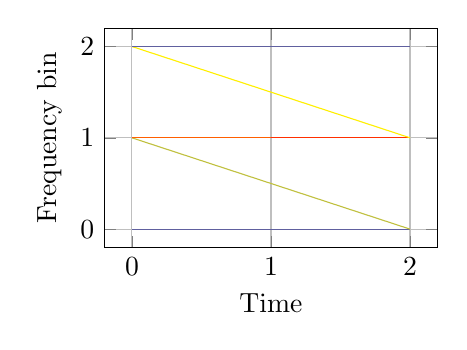
\begin{tikzpicture}
    \begin{axis}[
      width=0.48\textwidth,height=0.36\textwidth,
      xlabel={Time}, ylabel={Frequency bin}, grid=both]
      \addplot[mesh,draw=none,shader=interp,point meta=explicit] coordinates{ (0,0) [0.1] (1,0) [0.2] (2,0) [0.1]
        (0,1) [0.3] (1,1) [0.5] (2,1) [0.4]
        (0,2) [0.1] (1,2) [0.2] (2,2) [0.1] };
    \end{axis}
  \end{tikzpicture}
  \caption{Schematic spectrogram input for ASR.}
  \label{fig:asr-spec}
\end{figure}

\subsection{Text-to-Speech (TTS)}

Text-to-Speech (TTS) technology converts written text into natural-sounding speech, enabling applications that require audio output from text content. Modern TTS systems use neural vocoders and advanced synthesis techniques to generate speech that is virtually indistinguishable from human speech in terms of naturalness and expressiveness. The technology has evolved from robotic-sounding concatenative synthesis to sophisticated neural approaches that can capture the nuances of human speech, including emotion, intonation, and prosody. TTS systems are now integrated into a wide range of applications, from accessibility tools and virtual assistants to entertainment and educational content, making information more accessible and engaging for users with visual impairments or learning preferences.

WaveNet and Tacotron represent breakthrough architectures in neural TTS, using deep learning to generate high-quality speech from text input. WaveNet uses dilated convolutions to model the temporal dependencies in speech, producing more natural-sounding audio with better prosody and expressiveness. Tacotron combines sequence-to-sequence learning with attention mechanisms to generate mel-spectrograms from text, which are then converted to audio using neural vocoders. These architectures have enabled the development of voice synthesis systems that can mimic specific speakers, create custom voices for applications, and generate speech in multiple languages with native-like pronunciation. The technology has found applications in audiobook production, virtual assistants, and personalized voice interfaces.

Voice cloning technology has emerged as a powerful application of TTS, enabling the creation of synthetic voices that closely mimic specific individuals. This technology has applications in entertainment, where it can be used to create voiceovers for characters or restore the voices of actors who have passed away. In accessibility, voice cloning can help individuals with speech impairments create personalized synthetic voices that sound more natural and expressive than traditional text-to-speech systems. The technology has also found applications in language learning, where learners can practice pronunciation with native speaker voices, and in customer service, where synthetic voices can provide consistent and professional interactions. However, the technology also raises important ethical considerations regarding consent, privacy, and the potential for misuse in creating deepfake audio content.

Accessibility tools powered by TTS technology have transformed the lives of individuals with visual impairments, learning disabilities, and other conditions that affect reading ability. Screen readers use TTS to convert digital text into speech, enabling blind and visually impaired users to access websites, documents, and applications independently. Educational TTS systems can read textbooks, articles, and other learning materials aloud, supporting students with dyslexia and other reading difficulties. The technology has also enabled the creation of audiobooks and spoken content for entertainment and education, making information more accessible to diverse audiences. These tools continue to evolve, incorporating more natural-sounding voices, better pronunciation of technical terms, and support for multiple languages and accents.

\subsection{Speaker Recognition}

Speaker recognition technology identifies and verifies individuals based on their unique vocal characteristics, providing secure and convenient authentication methods. The technology analyzes various acoustic features of speech, including pitch, formants, and spectral characteristics, to create unique voiceprints for each individual. Modern speaker recognition systems use deep learning approaches to extract robust features that are resistant to noise, aging, and other factors that might affect voice quality. The technology has applications in security, authentication, and personalization, enabling hands-free access to devices and services. Speaker recognition is also used in forensic applications, where it can help identify individuals from audio recordings in criminal investigations.

Voice biometrics use speaker recognition technology to provide secure authentication for banking, healthcare, and other sensitive applications. Banks and financial institutions use voice biometrics to verify customer identity during phone calls, reducing fraud and improving security while maintaining convenience. Healthcare systems use voice authentication to secure access to patient records and medical devices, ensuring that only authorized personnel can access sensitive information. The technology has also found applications in smart home security, where it can recognize authorized users and grant access to restricted areas or functions. Voice biometrics offer several advantages over traditional authentication methods, including hands-free operation, resistance to spoofing attacks, and the ability to work across different devices and platforms.

Speaker diarization technology identifies who spoke when in multi-speaker conversations, providing valuable insights for meeting analysis, transcription, and content organization. The technology uses machine learning algorithms to segment audio recordings by speaker, enabling automatic identification of different participants in conversations. This capability is essential for accurate transcription of meetings, interviews, and other multi-speaker events, where it's important to know which person said what. Speaker diarization is also used in call center analytics, where it can help identify customer service representatives and customers in recorded calls for quality assurance and training purposes. The technology has applications in media production, where it can automatically identify and label different speakers in podcasts, interviews, and other audio content.

\subsection{Historical context and references}

The development of speech recognition and synthesis has been marked by several key breakthroughs that have transformed the field from rule-based systems to sophisticated neural architectures. The introduction of Hidden Markov Models (HMMs) in the 1970s provided the first statistical approach to speech recognition, enabling systems to learn from data rather than relying on hand-crafted rules. The development of Mel-Frequency Cepstral Coefficients (MFCCs) in the 1980s provided robust feature extraction methods that became the standard for speech processing systems. The introduction of neural networks in the 1990s marked a significant shift, with systems like TIMIT demonstrating the potential of deep learning for speech recognition tasks.

The 2000s saw the development of more sophisticated neural architectures, including Long Short-Term Memory (LSTM) networks and attention mechanisms that improved the ability to handle long sequences and complex speech patterns. The introduction of Connectionist Temporal Classification (CTC) in 2006 provided an efficient method for training sequence-to-sequence models without requiring frame-level alignments, making it easier to train ASR systems on large datasets. The development of WaveNet in 2016 marked a breakthrough in neural TTS, demonstrating that deep learning could generate high-quality speech that was virtually indistinguishable from human speech. The introduction of transformer architectures in 2017 further revolutionized the field, enabling more efficient processing of sequential data and better capture of long-range dependencies in speech.

The 2020s have seen the integration of self-supervised learning and large-scale pretraining, with models like wav2vec and Whisper demonstrating the power of learning from unlabeled audio data. These developments have made speech technology more accessible and cost-effective, enabling the development of systems that can work across multiple languages and domains with minimal labeled data. The field continues to evolve rapidly, with new architectures, training methods, and applications emerging regularly, making speech recognition and synthesis one of the most dynamic and impactful areas of artificial intelligence. See \textcite{Prince2023} for broader context and comprehensive tutorials on the theoretical foundations and practical applications of these transformative technologies.


% Chapter 12, Section 4

\section{Healthcare and Medical Imaging \difficultyInline{beginner}}
\label{sec:healthcare-applications}

\subsection{Medical Image Analysis}

\textbf{Disease detection:}
\begin{itemize}
    \item Cancer detection in mammograms, CT scans
    \item Diabetic retinopathy from retinal images
    \item Pneumonia detection from chest X-rays
\end{itemize}

\textbf{Segmentation:}
\begin{itemize}
    \item Tumor boundary delineation
    \item Organ segmentation for surgical planning
\end{itemize}

\subsection{Drug Discovery}

\begin{itemize}
    \item Predicting molecular properties
    \item Protein structure prediction (AlphaFold)
    \item Drug-target interaction prediction
\end{itemize}

\subsection{Clinical Decision Support}

\begin{itemize}
    \item Diagnosis assistance
    \item Treatment recommendation
    \item Risk prediction (readmission, mortality)
\end{itemize}

\subsection{Genomics}

% \subsection{Visual aids}
% \addcontentsline{toc}{subsubsection}{Visual aids (healthcare)}

% \begin{figure}[h]
%   \centering
%   \begin{tikzpicture}
%     \begin{axis}[
%       width=0.48\textwidth,height=0.36\textwidth,
%       xlabel={False Positive Rate}, ylabel={True Positive Rate},
%       xmin=0,xmax=1,ymin=0,ymax=1, grid=both]
%       \addplot[very thick,bookpurple] coordinates{(0,0) (0.1,0.7) (0.2,0.85) (0.4,0.92) (1,1)};
%       \addplot[bookpurple!40] coordinates{(0,0) (1,1)};
%     \end{axis}
%   \end{tikzpicture}
%   \caption{ROC curve schematic for a medical classifier.}
%   \label{fig:med-roc}
% \end{figure}

\subsection{Historical context and references}

CNNs enabled breakthroughs in segmentation and classification, notably U-Net in biomedical imaging \textcite{Ronneberger2015}. Clinical deployment emphasizes calibration and monitoring \textcite{Prince2023}.
\begin{itemize}
    \item DNA sequence analysis
    \item Variant calling
    \item Gene expression prediction
\end{itemize}


% Chapter 12, Section 5

\section{Reinforcement Learning Applications \difficultyInline{beginner}}
\label{sec:rl-applications}

Reinforcement learning represents one of the most exciting frontiers of artificial intelligence, where agents learn to make optimal decisions through trial and error in complex environments. Unlike supervised learning, which relies on labeled examples, reinforcement learning agents learn by interacting with their environment, receiving rewards or penalties for their actions, and gradually improving their decision-making strategies. This paradigm has enabled breakthrough achievements in game playing, robotics, autonomous systems, and resource optimization, demonstrating the power of learning from experience rather than explicit instruction. The technology has found applications in diverse domains, from entertainment and gaming to critical infrastructure and safety systems, where adaptive decision-making is essential for success. The integration of deep learning with reinforcement learning has created powerful systems that can master complex tasks and environments, opening new possibilities for artificial intelligence applications.

\subsection{Game Playing}

Game playing has been revolutionized by reinforcement learning, where AI agents have achieved superhuman performance in complex strategic games through self-play and deep learning. These systems learn optimal strategies by playing millions of games against themselves, gradually improving their decision-making through trial and error. The success of these systems has demonstrated the power of reinforcement learning to master complex, multi-step decision problems that require long-term planning and strategic thinking. These achievements have not only advanced the field of artificial intelligence but have also provided insights into human cognition and decision-making processes.

AlphaGo's victory over world champion Lee Sedol in 2016 marked a historic milestone in artificial intelligence, demonstrating that AI could master the ancient game of Go, which was considered too complex for computers. The system used deep neural networks combined with Monte Carlo tree search to evaluate board positions and plan moves, learning from millions of games played against itself. AlphaGo's success has inspired new approaches to strategic decision-making in various domains, from business strategy to military planning. The technology has also been applied to other complex games and strategic problems, demonstrating the versatility of reinforcement learning approaches for mastering challenging decision environments.

AlphaZero represents a breakthrough in general game-playing AI, demonstrating that a single algorithm could master multiple complex games without domain-specific knowledge. The system learned to play chess, shogi, and Go at superhuman levels by playing against itself, discovering novel strategies and playing styles that surprised human experts. AlphaZero's success has inspired new approaches to multi-domain learning and transfer learning, where knowledge gained in one domain can be applied to related problems. The technology has been applied to various strategic games and decision problems, demonstrating the power of general-purpose reinforcement learning algorithms for mastering complex environments.

OpenAI Five's success in Dota 2 demonstrated that reinforcement learning could master complex real-time strategy games that require teamwork, coordination, and long-term planning. The system learned to play the game at a professional level by training on thousands of games, developing sophisticated strategies and coordination patterns. OpenAI Five's achievements have inspired new approaches to multi-agent reinforcement learning and team coordination, where multiple AI agents must work together to achieve common goals. The technology has been applied to various multi-agent systems and collaborative AI applications, demonstrating the potential of reinforcement learning for complex, multi-agent environments.

AlphaStar's mastery of StarCraft II demonstrated that reinforcement learning could handle complex real-time strategy games with imperfect information and continuous action spaces. The system learned to play the game at a grandmaster level by training on millions of games, developing sophisticated strategies and micro-management skills. AlphaStar's success has inspired new approaches to real-time decision-making and resource management, where agents must make rapid decisions under uncertainty. The technology has been applied to various real-time systems and resource optimization problems, demonstrating the power of reinforcement learning for complex, dynamic environments.

\subsection{Robotics}

Robotics has been transformed by reinforcement learning, where robots learn to perform complex manipulation and navigation tasks through trial and error in real-world environments. These systems can adapt to changing conditions and learn new skills without explicit programming, making them more versatile and capable than traditional robotic systems. The technology has enabled robots to perform complex tasks in unstructured environments, from manufacturing and assembly to household chores and caregiving. These systems continue to evolve, with newer approaches incorporating simulation-to-real transfer and multi-modal learning to improve performance and generalization.

Manipulation tasks in robotics have been significantly improved by reinforcement learning, where robots learn to grasp, manipulate, and assemble objects through trial and error. These systems can adapt to different object shapes, sizes, and materials, learning optimal grasping strategies and manipulation techniques. The technology has been applied to manufacturing and assembly tasks, where robots must handle various products and components with high precision and reliability. These systems have been particularly valuable in flexible manufacturing environments, where robots must adapt to changing product requirements and production schedules. The technology continues to evolve, with newer approaches incorporating tactile feedback and multi-modal sensing to improve manipulation capabilities.

Navigation in robotics has been revolutionized by reinforcement learning, where robots learn to move autonomously through complex environments while avoiding obstacles and reaching their destinations. These systems can adapt to different environments and conditions, learning optimal navigation strategies and path-planning techniques. The technology has been applied to various robotic applications, from autonomous vehicles and drones to service robots and mobile platforms. These systems have been particularly valuable in dynamic environments, where robots must adapt to changing conditions and unexpected obstacles. The technology continues to evolve, with newer approaches incorporating advanced perception and planning capabilities to improve navigation performance.

Locomotion in robotics has been transformed by reinforcement learning, where robots learn to walk, run, and move in various ways through trial and error. These systems can adapt to different terrains and conditions, learning optimal locomotion strategies and movement patterns. The technology has been applied to various robotic applications, from humanoid robots and exoskeletons to quadruped robots and mobile platforms. These systems have been particularly valuable in challenging environments, where robots must adapt to rough terrain and changing conditions. The technology continues to evolve, with newer approaches incorporating advanced control and sensing capabilities to improve locomotion performance.

\subsection{Autonomous Vehicles}

Autonomous vehicles have been revolutionized by reinforcement learning, where AI systems learn to make complex driving decisions through trial and error in simulated and real-world environments. These systems can adapt to different driving conditions and scenarios, learning optimal driving strategies and decision-making techniques. The technology has been applied to various autonomous vehicle applications, from passenger cars and trucks to drones and autonomous ships. These systems have been particularly valuable in complex driving scenarios, where vehicles must make rapid decisions under uncertainty and changing conditions. The technology continues to evolve, with newer approaches incorporating advanced perception and planning capabilities to improve driving performance.

Path planning and decision making in autonomous vehicles have been significantly improved by reinforcement learning, where AI systems learn to plan optimal routes and make driving decisions through trial and error. These systems can adapt to different traffic conditions and scenarios, learning optimal driving strategies and decision-making techniques. The technology has been applied to various autonomous vehicle applications, from highway driving and city navigation to parking and maneuvering. These systems have been particularly valuable in complex driving scenarios, where vehicles must make rapid decisions under uncertainty and changing conditions. The technology continues to evolve, with newer approaches incorporating advanced perception and planning capabilities to improve driving performance.

The combination of reinforcement learning with computer vision has created powerful autonomous vehicle systems that can perceive their environment and make driving decisions based on visual information. These systems can identify and track other vehicles, pedestrians, and obstacles, enabling safe and efficient navigation through complex environments. The technology has been applied to various autonomous vehicle applications, from passenger cars and trucks to drones and autonomous ships. These systems have been particularly valuable in complex driving scenarios, where vehicles must make rapid decisions based on visual information and changing conditions. The technology continues to evolve, with newer approaches incorporating advanced perception and planning capabilities to improve driving performance.

Safety-critical systems in autonomous vehicles have been transformed by reinforcement learning, where AI systems learn to make safe driving decisions through trial and error in controlled environments. These systems can adapt to different safety requirements and scenarios, learning optimal safety strategies and decision-making techniques. The technology has been applied to various autonomous vehicle applications, from passenger cars and trucks to drones and autonomous ships. These systems have been particularly valuable in complex driving scenarios, where vehicles must make rapid decisions under uncertainty and changing conditions. The technology continues to evolve, with newer approaches incorporating advanced perception and planning capabilities to improve driving performance.

\subsection{Recommendation Systems}

Recommendation systems have been revolutionized by reinforcement learning, where AI systems learn to make personalized recommendations through trial and error in user interaction environments. These systems can adapt to different user preferences and behaviors, learning optimal recommendation strategies and decision-making techniques. The technology has been applied to various recommendation applications, from content and product recommendations to personalized services and experiences. These systems have been particularly valuable in dynamic environments, where user preferences and behaviors change over time. The technology continues to evolve, with newer approaches incorporating advanced user modeling and recommendation capabilities to improve performance.

Netflix and YouTube content recommendations have been transformed by reinforcement learning, where AI systems learn to recommend personalized content based on user behavior and preferences. These systems can adapt to different user tastes and viewing habits, learning optimal recommendation strategies and content selection techniques. The technology has been applied to various content recommendation applications, from movies and TV shows to music and podcasts. These systems have been particularly valuable in dynamic environments, where user preferences and content availability change over time. The technology continues to evolve, with newer approaches incorporating advanced user modeling and content analysis capabilities to improve recommendation performance.

E-commerce product suggestions have been significantly improved by reinforcement learning, where AI systems learn to recommend personalized products based on user behavior and preferences. These systems can adapt to different shopping patterns and preferences, learning optimal recommendation strategies and product selection techniques. The technology has been applied to various e-commerce applications, from online shopping and retail to marketplace and auction platforms. These systems have been particularly valuable in dynamic environments, where user preferences and product availability change over time. The technology continues to evolve, with newer approaches incorporating advanced user modeling and product analysis capabilities to improve recommendation performance.

Personalized news feeds have been transformed by reinforcement learning, where AI systems learn to recommend personalized news content based on user behavior and preferences. These systems can adapt to different reading habits and interests, learning optimal recommendation strategies and content selection techniques. The technology has been applied to various news and media applications, from social media and news aggregators to personalized content platforms. These systems have been particularly valuable in dynamic environments, where user interests and content availability change over time. The technology continues to evolve, with newer approaches incorporating advanced user modeling and content analysis capabilities to improve recommendation performance.

\subsection{Resource Management}

Resource management has been revolutionized by reinforcement learning, where AI systems learn to optimize resource allocation and utilization through trial and error in complex environments. These systems can adapt to different resource constraints and requirements, learning optimal management strategies and decision-making techniques. The technology has been applied to various resource management applications, from data center optimization and energy management to supply chain and logistics optimization. These systems have been particularly valuable in dynamic environments, where resource availability and demand change over time. The technology continues to evolve, with newer approaches incorporating advanced optimization and planning capabilities to improve resource management performance.

Data center cooling optimization has been transformed by reinforcement learning, where AI systems learn to optimize cooling systems and energy consumption through trial and error in data center environments. These systems can adapt to different cooling requirements and conditions, learning optimal cooling strategies and energy management techniques. The technology has been applied to various data center applications, from server cooling and energy management to facility optimization and maintenance. These systems have been particularly valuable in dynamic environments, where cooling requirements and energy costs change over time. The technology continues to evolve, with newer approaches incorporating advanced optimization and planning capabilities to improve cooling performance.

Traffic light control has been significantly improved by reinforcement learning, where AI systems learn to optimize traffic flow and reduce congestion through trial and error in traffic environments. These systems can adapt to different traffic patterns and conditions, learning optimal control strategies and traffic management techniques. The technology has been applied to various traffic management applications, from intersection control and signal optimization to traffic flow management and congestion reduction. These systems have been particularly valuable in dynamic environments, where traffic patterns and conditions change over time. The technology continues to evolve, with newer approaches incorporating advanced optimization and planning capabilities to improve traffic control performance.

Energy grid optimization has been transformed by reinforcement learning, where AI systems learn to optimize energy distribution and consumption through trial and error in power grid environments. These systems can adapt to different energy demands and supply conditions, learning optimal distribution strategies and energy management techniques. The technology has been applied to various energy management applications, from power grid optimization and renewable energy integration to energy storage and demand response. These systems have been particularly valuable in dynamic environments, where energy demand and supply change over time. The technology continues to evolve, with newer approaches incorporating advanced optimization and planning capabilities to improve energy management performance.

\subsection{Historical context and references}

The development of reinforcement learning has been marked by several key breakthroughs that have transformed the field from theoretical concepts to practical applications. The introduction of Q-learning in the 1980s provided the first practical algorithm for learning optimal policies in Markov decision processes, enabling agents to learn from experience without requiring a model of the environment. The development of policy gradient methods in the 1990s provided more efficient approaches to learning continuous control policies, enabling applications in robotics and autonomous systems. The introduction of deep reinforcement learning in the 2010s combined the power of deep neural networks with reinforcement learning, enabling agents to learn from high-dimensional sensory input and master complex environments.

The 2010s saw significant advances in reinforcement learning, with systems like DeepMind's AlphaGo demonstrating the power of deep reinforcement learning combined with tree search for mastering complex strategic games. The development of actor-critic methods and advanced policy gradient algorithms provided more stable and efficient approaches to learning complex policies. The introduction of experience replay and target networks improved the stability and efficiency of deep Q-learning, enabling applications in various domains. The development of multi-agent reinforcement learning opened new possibilities for collaborative AI and competitive environments.

The 2020s have seen the integration of reinforcement learning with other AI technologies, creating powerful systems that can learn from multiple modalities and adapt to complex environments. The development of transfer learning and meta-learning approaches has enabled agents to learn new tasks more efficiently by leveraging knowledge from related tasks. The integration of reinforcement learning with computer vision and natural language processing has created powerful systems that can understand and interact with complex environments. The field continues to evolve rapidly, with new algorithms, architectures, and applications emerging regularly, making reinforcement learning one of the most dynamic and impactful areas of artificial intelligence. See \textcite{Silver2016,Prince2023} for broader context and comprehensive tutorials on the theoretical foundations and practical applications of these transformative technologies.


% Chapter 12, Section 6

\section{Other Applications \difficultyInline{beginner}}
\label{sec:other-applications}

Beyond the major application domains of computer vision, natural language processing, speech recognition, healthcare, and reinforcement learning, deep learning has found transformative applications across numerous other sectors. These applications demonstrate the versatility and adaptability of deep learning technologies to diverse problems and industries, from financial services and scientific research to agriculture and manufacturing. The technology has enabled new approaches to complex problems that were previously intractable with traditional methods, opening up possibilities for innovation and efficiency gains across multiple sectors. These applications often require domain-specific adaptations and considerations, highlighting the importance of understanding both the technical capabilities of deep learning and the unique requirements of each application domain. The continued expansion of deep learning into new areas demonstrates its potential to transform industries and create new opportunities for technological advancement.

\subsection{Finance}

Finance has been revolutionized by deep learning applications that can analyze vast amounts of financial data to make predictions, detect patterns, and optimize trading strategies. These systems can process complex market data, news sentiment, and economic indicators to identify trading opportunities and manage risk more effectively than traditional methods. The technology has been particularly valuable for high-frequency trading, where rapid decision-making is essential for success. These systems continue to evolve, with newer approaches incorporating advanced risk management and regulatory compliance capabilities to improve performance and reliability.

Algorithmic trading has been transformed by deep learning systems that can analyze market data and execute trades with superhuman speed and accuracy. These systems can identify patterns in price movements, volume changes, and market sentiment to make profitable trading decisions. The technology has been applied to various financial markets, from stocks and bonds to commodities and currencies, enabling traders to capitalize on market opportunities more effectively. These systems have been particularly valuable for institutional investors and hedge funds, where they can process vast amounts of data and execute complex trading strategies. The technology continues to evolve, with newer approaches incorporating advanced risk management and regulatory compliance capabilities to improve trading performance.

Fraud detection has been significantly improved by deep learning models that can identify suspicious transactions and activities with high accuracy. These systems can analyze transaction patterns, user behavior, and other factors to detect fraudulent activities in real-time. The technology has been applied to various financial services, from credit cards and banking to insurance and investment platforms, helping to protect customers and reduce financial losses. These systems have been particularly valuable for online transactions and digital payments, where fraud risks are higher and traditional detection methods may be less effective. The technology continues to evolve, with newer approaches incorporating advanced behavioral analysis and anomaly detection capabilities to improve fraud prevention.

Credit risk assessment has been revolutionized by deep learning approaches that can analyze borrower characteristics and predict default probabilities with high accuracy. These systems can process various types of data, from credit scores and income statements to social media activity and spending patterns, to assess creditworthiness. The technology has been applied to various lending applications, from personal loans and mortgages to business credit and investment decisions, enabling more accurate risk assessment and pricing. These systems have been particularly valuable for alternative lending and fintech applications, where traditional credit assessment methods may be less effective. The technology continues to evolve, with newer approaches incorporating advanced behavioral analysis and alternative data sources to improve credit assessment accuracy.

Market prediction has been transformed by deep learning models that can forecast price movements and market trends with improved accuracy. These systems can analyze various factors, from economic indicators and news sentiment to technical analysis and market microstructure, to predict future market behavior. The technology has been applied to various financial markets, from stocks and bonds to commodities and currencies, enabling investors to make more informed decisions. These systems have been particularly valuable for portfolio management and risk assessment, where accurate market predictions are essential for success. The technology continues to evolve, with newer approaches incorporating advanced time series analysis and multi-modal data processing to improve prediction accuracy.

\subsection{Scientific Research}

Scientific research has been transformed by deep learning applications that can analyze complex data and identify patterns that may be difficult for human researchers to detect. These systems can process vast amounts of experimental data, simulations, and observations to discover new insights and accelerate the pace of scientific discovery. The technology has been applied to various scientific disciplines, from physics and chemistry to biology and environmental science, enabling researchers to tackle complex problems more effectively. These systems continue to evolve, with newer approaches incorporating advanced data analysis and pattern recognition capabilities to improve scientific research outcomes.

Physics research has been revolutionized by deep learning applications that can analyze particle physics data and detect gravitational waves with unprecedented sensitivity. These systems can process complex experimental data to identify particle interactions, classify events, and detect rare phenomena that may be missed by traditional analysis methods. The technology has been applied to various physics experiments, from particle accelerators and detectors to gravitational wave observatories and neutrino experiments, enabling researchers to discover new particles and phenomena. These systems have been particularly valuable for high-energy physics experiments, where vast amounts of data must be processed to identify rare events and interactions. The technology continues to evolve, with newer approaches incorporating advanced signal processing and pattern recognition capabilities to improve physics research outcomes.

Climate science has been transformed by deep learning models that can analyze climate data and predict weather patterns with improved accuracy. These systems can process various types of data, from satellite imagery and weather stations to ocean currents and atmospheric conditions, to forecast weather and climate changes. The technology has been applied to various climate applications, from weather forecasting and climate modeling to extreme weather prediction and climate change analysis, enabling researchers to better understand and predict climate behavior. These systems have been particularly valuable for long-term climate projections and extreme weather events, where accurate predictions are essential for planning and preparedness. The technology continues to evolve, with newer approaches incorporating advanced data assimilation and multi-scale modeling to improve climate prediction accuracy.

Astronomy has been revolutionized by deep learning applications that can analyze astronomical data and identify celestial objects with superhuman accuracy. These systems can process images from telescopes and observatories to classify galaxies, detect exoplanets, and identify other astronomical phenomena. The technology has been applied to various astronomical surveys, from galaxy classification and exoplanet detection to supernova identification and gravitational lensing analysis, enabling researchers to discover new celestial objects and phenomena. These systems have been particularly valuable for large-scale astronomical surveys, where vast amounts of data must be processed to identify rare and interesting objects. The technology continues to evolve, with newer approaches incorporating advanced image processing and pattern recognition capabilities to improve astronomical research outcomes.

\subsection{Agriculture}

Agriculture has been transformed by deep learning applications that can analyze crop data and optimize farming practices to improve yields and reduce environmental impact. These systems can process various types of data, from satellite imagery and weather data to soil conditions and crop health, to provide farmers with actionable insights and recommendations. The technology has been applied to various agricultural applications, from crop monitoring and disease detection to yield prediction and precision agriculture, enabling farmers to make more informed decisions and improve productivity. These systems have been particularly valuable for large-scale farming operations, where data-driven insights can significantly impact profitability and sustainability. The technology continues to evolve, with newer approaches incorporating advanced sensor data and machine learning capabilities to improve agricultural outcomes.

Crop disease detection has been revolutionized by deep learning models that can identify plant diseases and pests with high accuracy from images and sensor data. These systems can analyze various types of data, from drone imagery and satellite photos to ground-based sensors and weather data, to detect diseases early and recommend treatment strategies. The technology has been applied to various crops, from wheat and corn to fruits and vegetables, enabling farmers to prevent disease outbreaks and minimize crop losses. These systems have been particularly valuable for organic farming and sustainable agriculture, where early disease detection is essential for maintaining crop health without chemical treatments. The technology continues to evolve, with newer approaches incorporating advanced image processing and sensor fusion to improve disease detection accuracy.

Yield prediction has been significantly improved by deep learning approaches that can forecast crop yields with high accuracy based on various factors. These systems can analyze weather data, soil conditions, planting patterns, and historical yields to predict future harvests and optimize farming decisions. The technology has been applied to various crops and farming systems, from traditional agriculture to precision farming and vertical farming, enabling farmers to plan their operations more effectively. These systems have been particularly valuable for commodity trading and food security planning, where accurate yield predictions are essential for market stability and food supply management. The technology continues to evolve, with newer approaches incorporating advanced weather modeling and soil analysis to improve yield prediction accuracy.

Precision agriculture has been transformed by deep learning systems that can optimize farming practices at the individual plant or field level. These systems can analyze various types of data, from soil sensors and weather stations to drone imagery and satellite data, to provide personalized recommendations for each part of a field. The technology has been applied to various farming operations, from crop planting and fertilization to irrigation and harvesting, enabling farmers to maximize yields while minimizing resource use. These systems have been particularly valuable for sustainable farming and environmental conservation, where precision agriculture can reduce water usage, fertilizer application, and environmental impact. The technology continues to evolve, with newer approaches incorporating advanced robotics and automation to improve precision agriculture outcomes.

\subsection{Manufacturing}

Manufacturing has been revolutionized by deep learning applications that can optimize production processes, detect defects, and predict maintenance needs with unprecedented accuracy. These systems can analyze various types of data, from production sensors and quality control measurements to supply chain information and customer feedback, to improve manufacturing efficiency and product quality. The technology has been applied to various manufacturing processes, from automotive and electronics to pharmaceuticals and food production, enabling companies to reduce costs and improve competitiveness. These systems have been particularly valuable for high-volume manufacturing operations, where small improvements in efficiency can have significant impact on profitability. The technology continues to evolve, with newer approaches incorporating advanced robotics and automation to improve manufacturing outcomes.

Quality control and defect detection have been transformed by deep learning models that can identify product defects and quality issues with superhuman accuracy. These systems can analyze various types of data, from visual inspections and sensor measurements to production parameters and test results, to detect defects early and prevent quality issues. The technology has been applied to various manufacturing processes, from automotive assembly and electronics production to pharmaceutical manufacturing and food processing, enabling companies to maintain high quality standards and reduce waste. These systems have been particularly valuable for automated production lines, where real-time quality control is essential for maintaining product consistency and customer satisfaction. The technology continues to evolve, with newer approaches incorporating advanced computer vision and sensor fusion to improve quality control accuracy.

Predictive maintenance has been significantly improved by deep learning approaches that can predict equipment failures and maintenance needs with high accuracy. These systems can analyze various types of data, from vibration sensors and temperature readings to production parameters and historical maintenance records, to forecast when equipment will need maintenance or replacement. The technology has been applied to various manufacturing equipment, from motors and pumps to conveyor belts and robotic systems, enabling companies to prevent unplanned downtime and reduce maintenance costs. These systems have been particularly valuable for critical manufacturing processes, where equipment failures can cause significant production losses and safety risks. The technology continues to evolve, with newer approaches incorporating advanced sensor data and machine learning capabilities to improve predictive maintenance accuracy.

Supply chain optimization has been revolutionized by deep learning systems that can optimize supply chain operations and predict demand patterns with improved accuracy. These systems can analyze various types of data, from sales forecasts and inventory levels to supplier performance and transportation costs, to optimize supply chain decisions and reduce costs. The technology has been applied to various supply chain applications, from inventory management and demand forecasting to supplier selection and logistics optimization, enabling companies to improve efficiency and reduce supply chain risks. These systems have been particularly valuable for global supply chains, where complex logistics and demand variability can significantly impact costs and service levels. The technology continues to evolve, with newer approaches incorporating advanced optimization algorithms and real-time data processing to improve supply chain performance.

\subsection{References}

For domain-specific overviews, see \textcite{Prince2023} (applications survey). The applications discussed in this section represent just a sample of the diverse ways in which deep learning is transforming industries and creating new opportunities for technological advancement. These applications demonstrate the versatility and adaptability of deep learning technologies to diverse problems and industries, from financial services and scientific research to agriculture and manufacturing. The continued expansion of deep learning into new areas demonstrates its potential to transform industries and create new opportunities for technological advancement. As the field continues to evolve, we can expect to see even more innovative applications and breakthroughs that will further demonstrate the power and potential of deep learning technologies.


% Chapter 12: Real World Applications

\section{Real World Applications}
\label{sec:applications-real-world}


While this chapter already discusses many applications, this section provides additional concrete examples of how deep learning technologies integrate into everyday products and services.

\subsection{Smart Home Devices}

Deep learning makes homes more intelligent and responsive:

\begin{itemize}
    \item \textbf{Smart speakers with voice control:} Devices like Amazon Echo and Google Home use multiple deep learning models working together: speech recognition converts your voice to text, natural language understanding interprets your intent, and text-to-speech responds naturally. These run locally for privacy while cloud models handle complex queries.
    
    \item \textbf{Energy optimization:} Smart thermostats learn your schedule and preferences, using sequence models to predict when you'll be home and adjusting temperature efficiently. This saves energy while maintaining comfort, learning patterns like "weekday mornings" versus "weekend sleep-ins."
    
    \item \textbf{Security cameras with intelligent alerts:} Instead of alerting you to every motion, smart cameras use computer vision to distinguish between family members, delivery people, and potential intruders. They can even recognize familiar faces and alert you only to unexpected visitors.
\end{itemize}

\subsection{Entertainment and Media}

Personalized content discovery and creation:

\begin{itemize}
    \item \textbf{Music streaming personalization:} Spotify's Discover Weekly and similar features use deep learning to analyze your listening habits, finding new music matching your taste. Models consider factors like song characteristics, listening context (workout versus relaxation), and discovery patterns of similar users.
    
    \item \textbf{Video game AI:} Modern games use deep learning for realistic non-player character behavior, procedural content generation, and adaptive difficulty. Racing games learn from your driving style to provide challenging but fair opponents; strategy games develop tactics matching your skill level.
    
    \item \textbf{Content creation tools:} Apps that remove backgrounds from photos, enhance low-light images, or create artistic filters all use deep learning. Tools like DALL-E and Midjourney enable anyone to create visual content from text descriptions, democratizing digital art creation.
\end{itemize}

\subsection{Agriculture and Food Production}

Feeding the world more efficiently:

\begin{itemize}
    \item \textbf{Crop disease detection:} Farmers photograph plants with smartphones; deep learning identifies diseases early when treatment is most effective. This reduces crop losses and chemical use, as farmers apply pesticides only where needed rather than entire fields.
    
    \item \textbf{Autonomous farming equipment:} Tractors and harvesters using computer vision navigate fields autonomously, optimize planting patterns, and identify weeds for precision herbicide application. This increases yields while reducing environmental impact and labor costs.
    
    \item \textbf{Food quality inspection:} Processing facilities use vision systems to inspect products at superhuman speeds—checking eggs for cracks, sorting fruits by ripeness, detecting foreign objects in packaged foods. This improves food safety while reducing waste from over-cautious human inspection.
\end{itemize}

\subsection{Integration and Impact}

What makes these applications successful:
\begin{itemize}
    \item \textbf{Seamless integration:} AI works invisibly, enhancing rather than complicating user experience
    \item \textbf{Continuous improvement:} Systems learn from usage, becoming more personalized over time
    \item \textbf{Practical constraints:} Solutions balance accuracy, speed, cost, and privacy appropriately
    \item \textbf{Accessibility:} Advanced AI capabilities available through consumer devices
\end{itemize}

These examples illustrate how deep learning pervades modern life, often working behind the scenes to make products smarter, more efficient, and more personalized.

% Index entries
\index{applications!smart home}
\index{applications!entertainment}
\index{applications!agriculture}
\index{applications!integration}

% Chapter 12, Section 7

\section{Ethical Considerations \difficultyInline{beginner}}
\label{sec:ethics}

Deep learning applications raise important ethical concerns that must be carefully considered and addressed throughout the development and deployment process. These concerns span multiple dimensions, from technical challenges like bias and transparency to broader societal impacts like job displacement and environmental sustainability. As deep learning systems become more powerful and widely deployed, the ethical implications of their use become increasingly significant, requiring proactive measures to ensure responsible development and deployment. The field has recognized the importance of ethical considerations, with researchers, practitioners, and organizations developing frameworks, guidelines, and best practices to address these challenges. Responsible AI development requires addressing these challenges through comprehensive documentation, human oversight, continuous monitoring, and careful consideration of environmental costs during model selection.

Bias and fairness represent critical ethical concerns in deep learning applications, where models may perpetuate or amplify societal biases present in training data. These biases can manifest in various ways, from discriminatory hiring decisions in automated screening systems to unfair loan approvals in financial applications, potentially reinforcing existing inequalities and creating new forms of discrimination. The challenge is particularly acute because bias can be subtle and difficult to detect, especially in complex deep learning models that process high-dimensional data and make decisions through non-linear transformations. Addressing bias requires careful attention to data collection and preprocessing, diverse and representative training datasets, and ongoing monitoring of model performance across different demographic groups. The field has developed various techniques for bias detection and mitigation, including fairness constraints, adversarial debiasing, and post-processing methods, though achieving true fairness remains an ongoing challenge that requires both technical and social solutions.

Privacy concerns have become increasingly prominent as deep learning systems process vast amounts of personal data, from medical records and financial information to social media posts and location data. These systems can extract sensitive information from seemingly innocuous data, creating risks for individual privacy and data protection. The challenge is compounded by the fact that deep learning models can memorize training data and potentially leak sensitive information through their outputs or intermediate representations. Privacy-preserving techniques such as differential privacy, federated learning, and secure multi-party computation have been developed to address these concerns, but implementing them effectively while maintaining model performance remains challenging. Organizations must carefully balance the benefits of data-driven insights with the need to protect individual privacy, often requiring legal compliance with regulations like GDPR and CCPA while implementing technical safeguards.

Transparency and interpretability represent fundamental challenges in deep learning, where the "black box" nature of complex models makes it difficult to understand how decisions are made. This lack of transparency can be problematic in high-stakes applications like healthcare, finance, and criminal justice, where understanding the reasoning behind decisions is crucial for trust, accountability, and regulatory compliance. The challenge is particularly acute for deep learning models, which often have millions of parameters and make decisions through complex, non-linear transformations that are difficult to interpret. Various techniques have been developed to improve model interpretability, including attention mechanisms, gradient-based methods, and surrogate models, but achieving full transparency while maintaining model performance remains an ongoing challenge. The field continues to evolve, with new approaches to explainable AI and interpretable machine learning being developed to address these concerns.

Security vulnerabilities in deep learning systems represent a significant ethical concern, where models can be manipulated through adversarial attacks and other malicious techniques. These attacks can cause models to make incorrect predictions or decisions, potentially leading to safety risks, financial losses, or other harmful outcomes. The challenge is particularly concerning for safety-critical applications like autonomous vehicles, medical diagnosis, and financial systems, where adversarial attacks could have serious consequences. Adversarial training, robust optimization, and other defensive techniques have been developed to improve model security, but achieving robust security while maintaining model performance remains challenging. The field continues to evolve, with new approaches to adversarial robustness and secure machine learning being developed to address these concerns.

Job displacement represents a significant societal concern as deep learning systems automate tasks previously performed by humans, potentially leading to unemployment and economic disruption. This displacement can affect workers across various industries, from manufacturing and transportation to healthcare and finance, creating challenges for individuals, communities, and society as a whole. The challenge is particularly acute because automation can affect both routine and non-routine tasks, potentially displacing workers who may lack the skills or resources to transition to new roles. Addressing job displacement requires proactive measures, including education and training programs, social safety nets, and policies that support workers through transitions. The field has recognized the importance of responsible automation, with researchers and practitioners developing frameworks and guidelines to ensure that AI deployment benefits society as a whole.

Environmental impact has become an increasingly important ethical consideration as deep learning models become larger and more computationally intensive, requiring significant energy consumption for training and inference. The environmental cost of large models can be substantial, with some models requiring energy equivalent to that used by small cities, raising concerns about sustainability and climate change. The challenge is particularly acute for large language models and other resource-intensive applications, where the environmental cost of training and deployment can be significant. Addressing environmental impact requires careful consideration of model efficiency, renewable energy sources, and the trade-offs between model performance and environmental cost. The field has developed various techniques for efficient model design, including model compression, quantization, and knowledge distillation, though achieving optimal efficiency while maintaining performance remains an ongoing challenge.

% \subsection{Visual aids}
% \addcontentsline{toc}{subsubsection}{Visual aids (ethics)}

% \begin{figure}[h]
%   \centering
%   \begin{tikzpicture}
%     \begin{axis}[
%       width=0.48\textwidth,height=0.36\textwidth,
%       ybar, bar width=12pt, grid=both,
%       xlabel={Concern}, ylabel={Priority (example)}, xtick=data,
%       xticklabels={Bias,Privacy,Security,Transparency,Environment}]
%       \addplot[bookred,fill=bookred!40] coordinates{(1,9) (2,8) (3,7) (4,7) (5,6)};
%     \end{axis}
%   \end{tikzpicture}
%   \caption{Example prioritization of ethical concerns (illustrative).}
%   \label{fig:ethics-priority}
% \end{figure}


% Chapter summary and problems
% Key Takeaways for Chapter 12

\section*{Key Takeaways}
\addcontentsline{toc}{section}{Key Takeaways}

\begin{keytakeaways}
\begin{itemize}[leftmargin=2em]
    \item \textbf{Domain-specific applications}: Deep learning has transformed computer vision, NLP, speech recognition, healthcare, and reinforcement learning, with each domain requiring specialized architectures and approaches tailored to specific data types and constraints.
    \item \textbf{Real-world impact}: Applications span from entertainment and gaming to critical infrastructure and safety systems, demonstrating the versatility of deep learning across diverse industries including finance, scientific research, agriculture, and manufacturing.
    \item \textbf{Systematic approach}: Successful applications require understanding the fundamental characteristics of each domain, including data assumptions, evaluation metrics, and deployment considerations, before selecting appropriate model families and training strategies.
    \item \textbf{Ethical responsibility}: As deep learning systems become more powerful and widely deployed, addressing bias, privacy, transparency, security, job displacement, and environmental impact becomes crucial for responsible AI development.
    \item \textbf{Practical constraints}: Real-world success depends on balancing technical sophistication with practical constraints, often achieving better results through careful problem formulation and data understanding than through complex model architectures.
\end{itemize}
\end{keytakeaways}



% Exercises (Exercises) for Chapter 12

\section*{Exercises}
\addcontentsline{toc}{section}{Exercises}

\subsection*{Easy}

\begin{problem}[Vision Metrics]
Choose between accuracy, AUROC, and mAP for object detection. Justify.

\textbf{Hint:} Class imbalance and localisation vs. classification.
\end{problem}

\begin{problem}[NLP Tokenisation]
Explain implications of BPE vs. WordPiece for rare words.

\textbf{Hint:} Subword frequency, OOV handling, sequence length.
\end{problem}

\begin{problem}[Tabular Baselines]
Why can tree ensembles outperform deep nets on small tabular datasets?

\textbf{Hint:} Inductive bias, feature interactions, sample efficiency.
\end{problem}

\begin{problem}[Data Privacy]
List two privacy risks when deploying medical models and mitigations.

\textbf{Hint:} Re-identification, membership inference; anonymisation, DP.
\end{problem}

\subsection*{Medium}

\begin{problem}[Dataset Shift]
Design a test to detect covariate shift between training and production.

\textbf{Hint:} Train a domain classifier; compare feature distributions.
\end{problem}

\begin{problem}[Active Learning]
Propose an acquisition strategy for labelling a limited budget.

\textbf{Hint:} Uncertainty sampling, diversity, class balance.
\end{problem}

\subsection*{Hard}

\begin{problem}[Cost-aware Serving]
Formalise an objective trading accuracy vs. compute cost and latency.

\textbf{Hint:} Multi-objective optimisation; constrained maximisation.
\end{problem}

\begin{problem}[Ethical Deployment]
Specify post-deployment monitoring and escalation for high-stakes tasks.

\textbf{Hint:} Thresholds, audits, rollback, human oversight.
\end{problem}



\begin{problem}[Advanced Topic 1]
Explain a key concept from this chapter and its practical applications.

\textbf{Hint:} Consider the theoretical foundations and real-world implications.
\end{problem}

\begin{problem}[Advanced Topic 2]
Analyse the relationship between different techniques covered in this chapter.

\textbf{Hint:} Look for connections and trade-offs between methods.
\end{problem}

\begin{problem}[Advanced Topic 3]
Design an experiment to test a hypothesis related to this chapter's content.

\textbf{Hint:} Consider experimental design, metrics, and potential confounding factors.
\end{problem}

\begin{problem}[Advanced Topic 4]
Compare different approaches to solving a problem from this chapter.

\textbf{Hint:} Consider computational complexity, accuracy, and practical considerations.
\end{problem}

\begin{problem}[Advanced Topic 5]
Derive a mathematical relationship or prove a theorem from this chapter.

\textbf{Hint:} Start with the definitions and work through the logical steps.
\end{problem}

\begin{problem}[Advanced Topic 6]
Implement a practical solution to a problem discussed in this chapter.

\textbf{Hint:} Consider the implementation details and potential challenges.
\end{problem}

\begin{problem}[Advanced Topic 7]
Evaluate the limitations and potential improvements of techniques from this chapter.

\textbf{Hint:} Consider both theoretical limitations and practical constraints.
\end{problem}

